\documentclass{jarticle}
\usepackage[dvipdfmx]{graphicx}

\title{ソフトウェア設計及び実験\\レポート作成の練習課題}
\author{6119019056 山口力也}
\date{2019/04/09}

\begin{document}
\maketitle

\section{実習の目的}
実習の目的は以下のとおりである.\\
\begin{itemize}

\item \LaTeX の使い方を習得する.
\item gnuplotの使い方を習得する.
\item Diaの使い方を習得する.

\end{itemize}
なお、\LaTeX の詳細については,参考文献\cite{okumura},\cite{matsuda}などを参照すること.


\section{原理・アルゴリズム}
\subsection{Diaで作成した図の挿入}
図\ref{fig:dia}は,Diaで作成したポストスクリプトファイルを挿入したものである.


\begin{figure}
\begin{center}
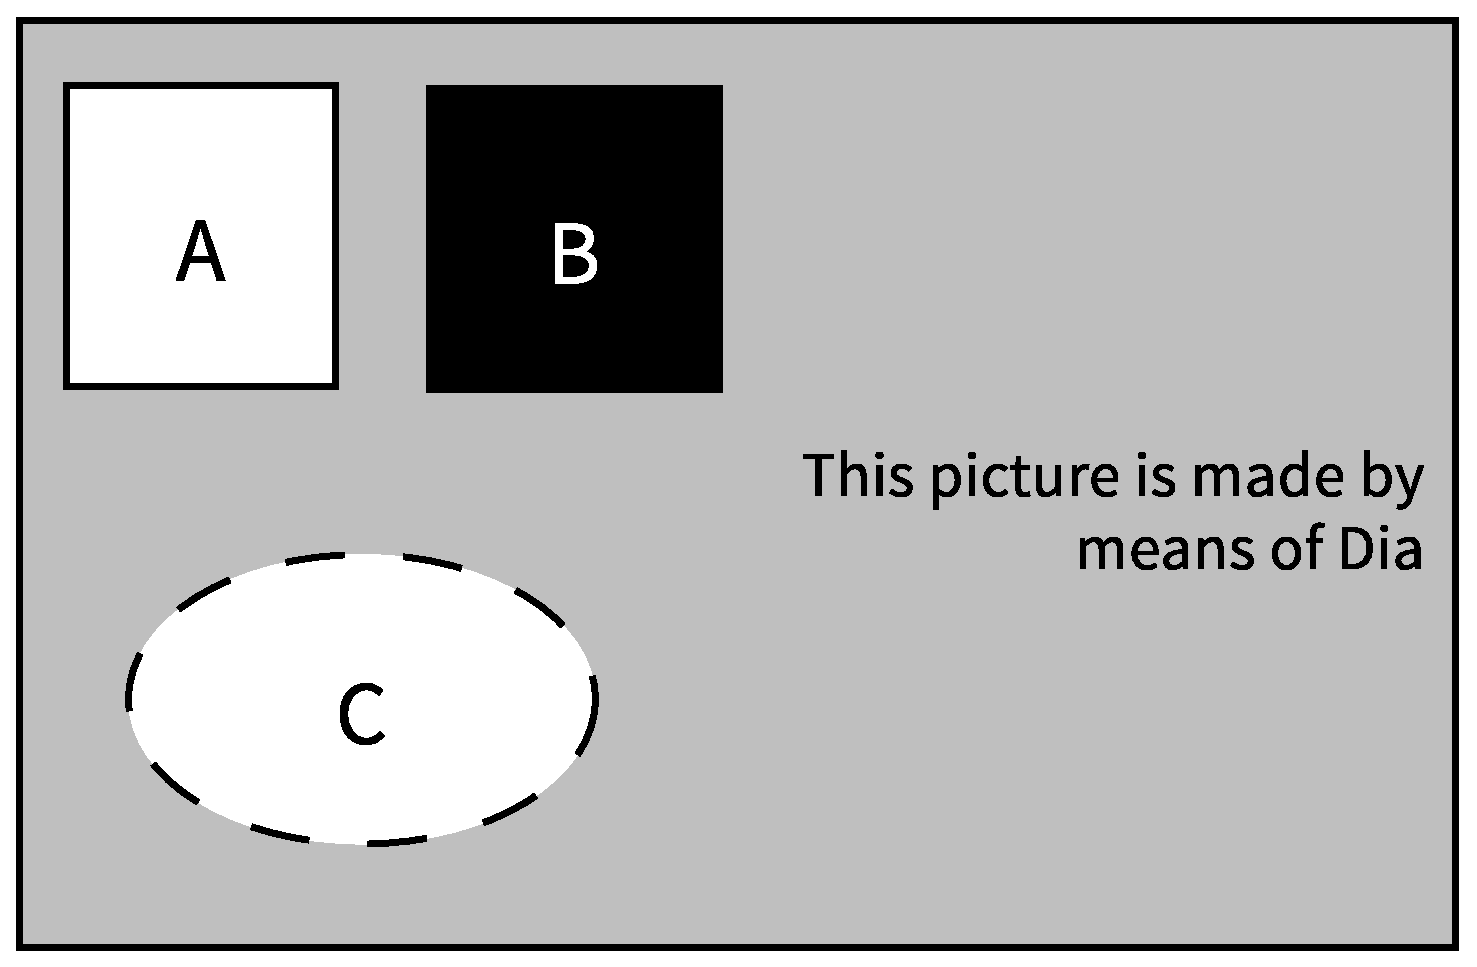
\includegraphics[width=8.0cm]{dia.eps}
\caption{Diaにより作成された図}
\label{fig:dia}
\end{center}
\end{figure}

\subsection{gnuplotで作成した図の挿入}
図\ref{fig:graph}は,ファイル"datafile"中の数値をgnuplotでグラフ化した後,Diaで加工した図を挿入したものである.

\begin{figure}
\begin{center}
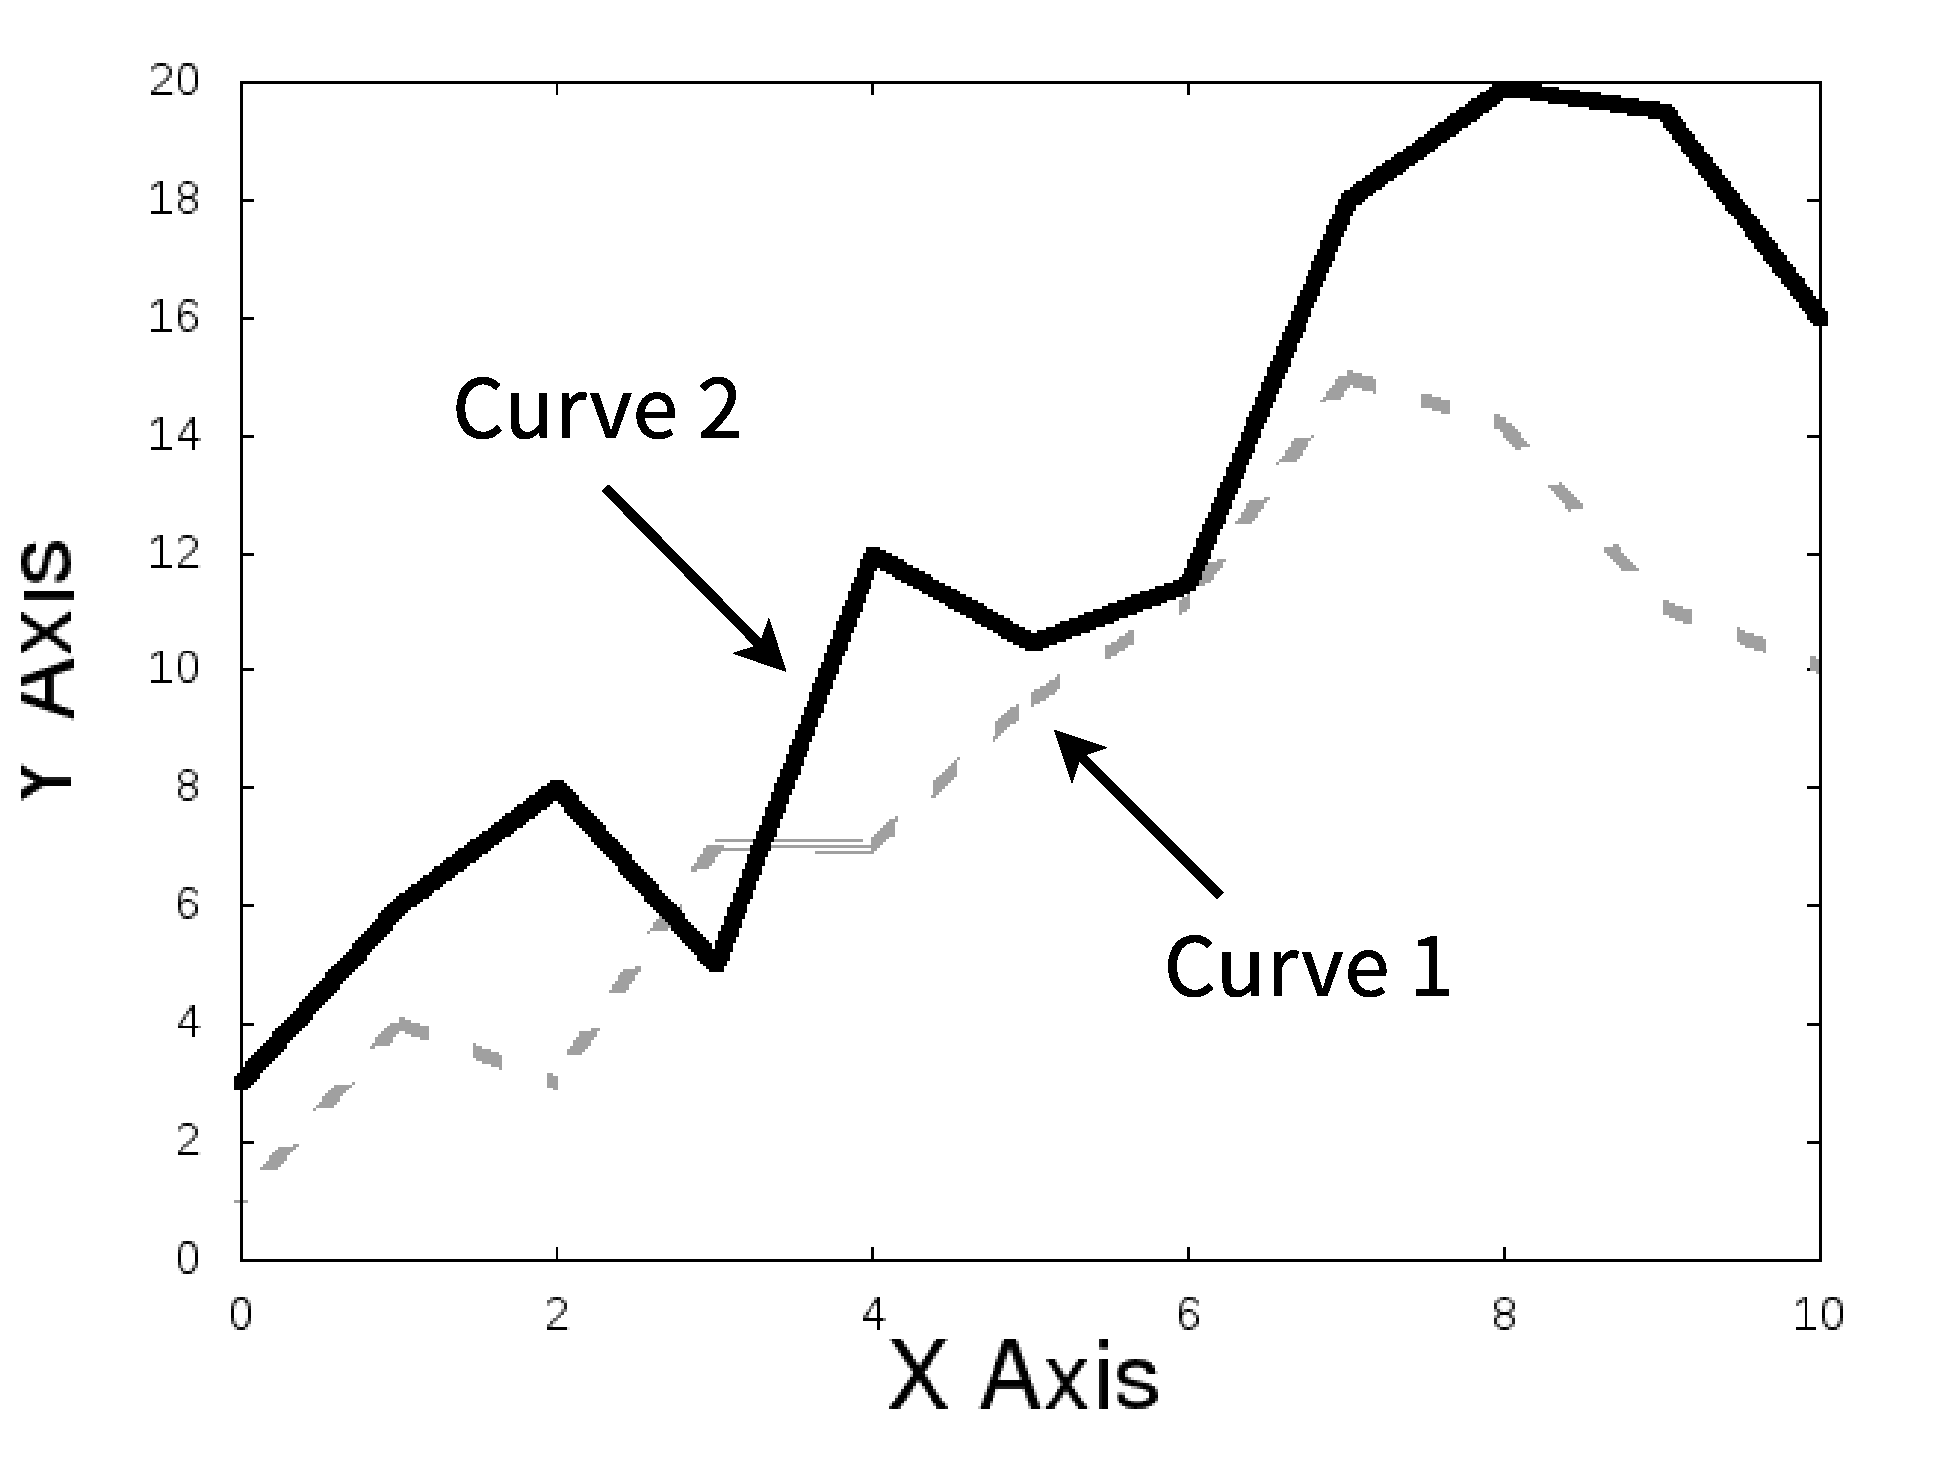
\includegraphics[width=8.0cm]{graph-e.eps}
\caption{gnuplotとDiaを用いて作成された図の挿入例}
\label{fig:graph}
\end{center}
\end{figure}

\section{表を作成する練習}
表\ref{table:datafile}は、ファイル"datafile"の数値を表にまとめたものである.


\begin{table}
\caption{表の例}
\label{table:datafile}
\begin{center}
\begin{tabular}{|c|c|c|}\hline
$x$ & $y_{1}$ & $y_{2}$ \\ \hline
0.0 & 1.0 & 3.0 \\ \hline
1.0 & 4.0 & 6.0 \\ \hline
2.0 & 3.0 & 8.0 \\ \hline
3.0 & 7.0 & 5.0 \\\hline
4.0 & 7.0 & 12.0 \\\hline
5.0 & 9.5 & 10.5 \\\hline
6.0 & 11.2 & 11.5 \\\hline
7.0 & 15.0 & 18.0 \\\hline
8.0 & 14.2 & 19.9 \\\hline
9.0 & 11.1 & 19.5 \\\hline
10.0 & 10.1 & 16.0 \\\hline
\end{tabular}
\end{center}
\end{table}
\section{本実験に対する意気込みなど}
編入生ということで一つ下の学年の子と一緒に実験をすることになるので,他の子を先導しつつ,能動的に色々なことにチャレンジしたい.
\

\begin{thebibliography}{99}
%
\bibitem{okumura} 奥村 晴彦: LaTeX2ε美文書作成入門 改訂第4版,  技術評論社 (2006).
%
\bibitem{matsuda} 松田七美男 : Linux活用術, 東京電機大学出版局 (1998).
%
\end{thebibliography}
end{document}

